\documentclass{article}

\usepackage{graphicx}
\usepackage{tikz}
\usepackage{tikzsymbols}
\usetikzlibrary{calc,patterns,shapes.geometric}
\pagestyle{empty}
\usepackage[margin=0pt]{geometry}
\geometry{papersize={14in,12in}}

\def\centerarc[#1](#2)(#3:#4:#5){\draw[#1] ($(#2)+({#5*cos(#3)},{#5*sin(#3)})$) arc (#3:#4:#5);}

\begin{document}
	\begin{figure}
		\centering
		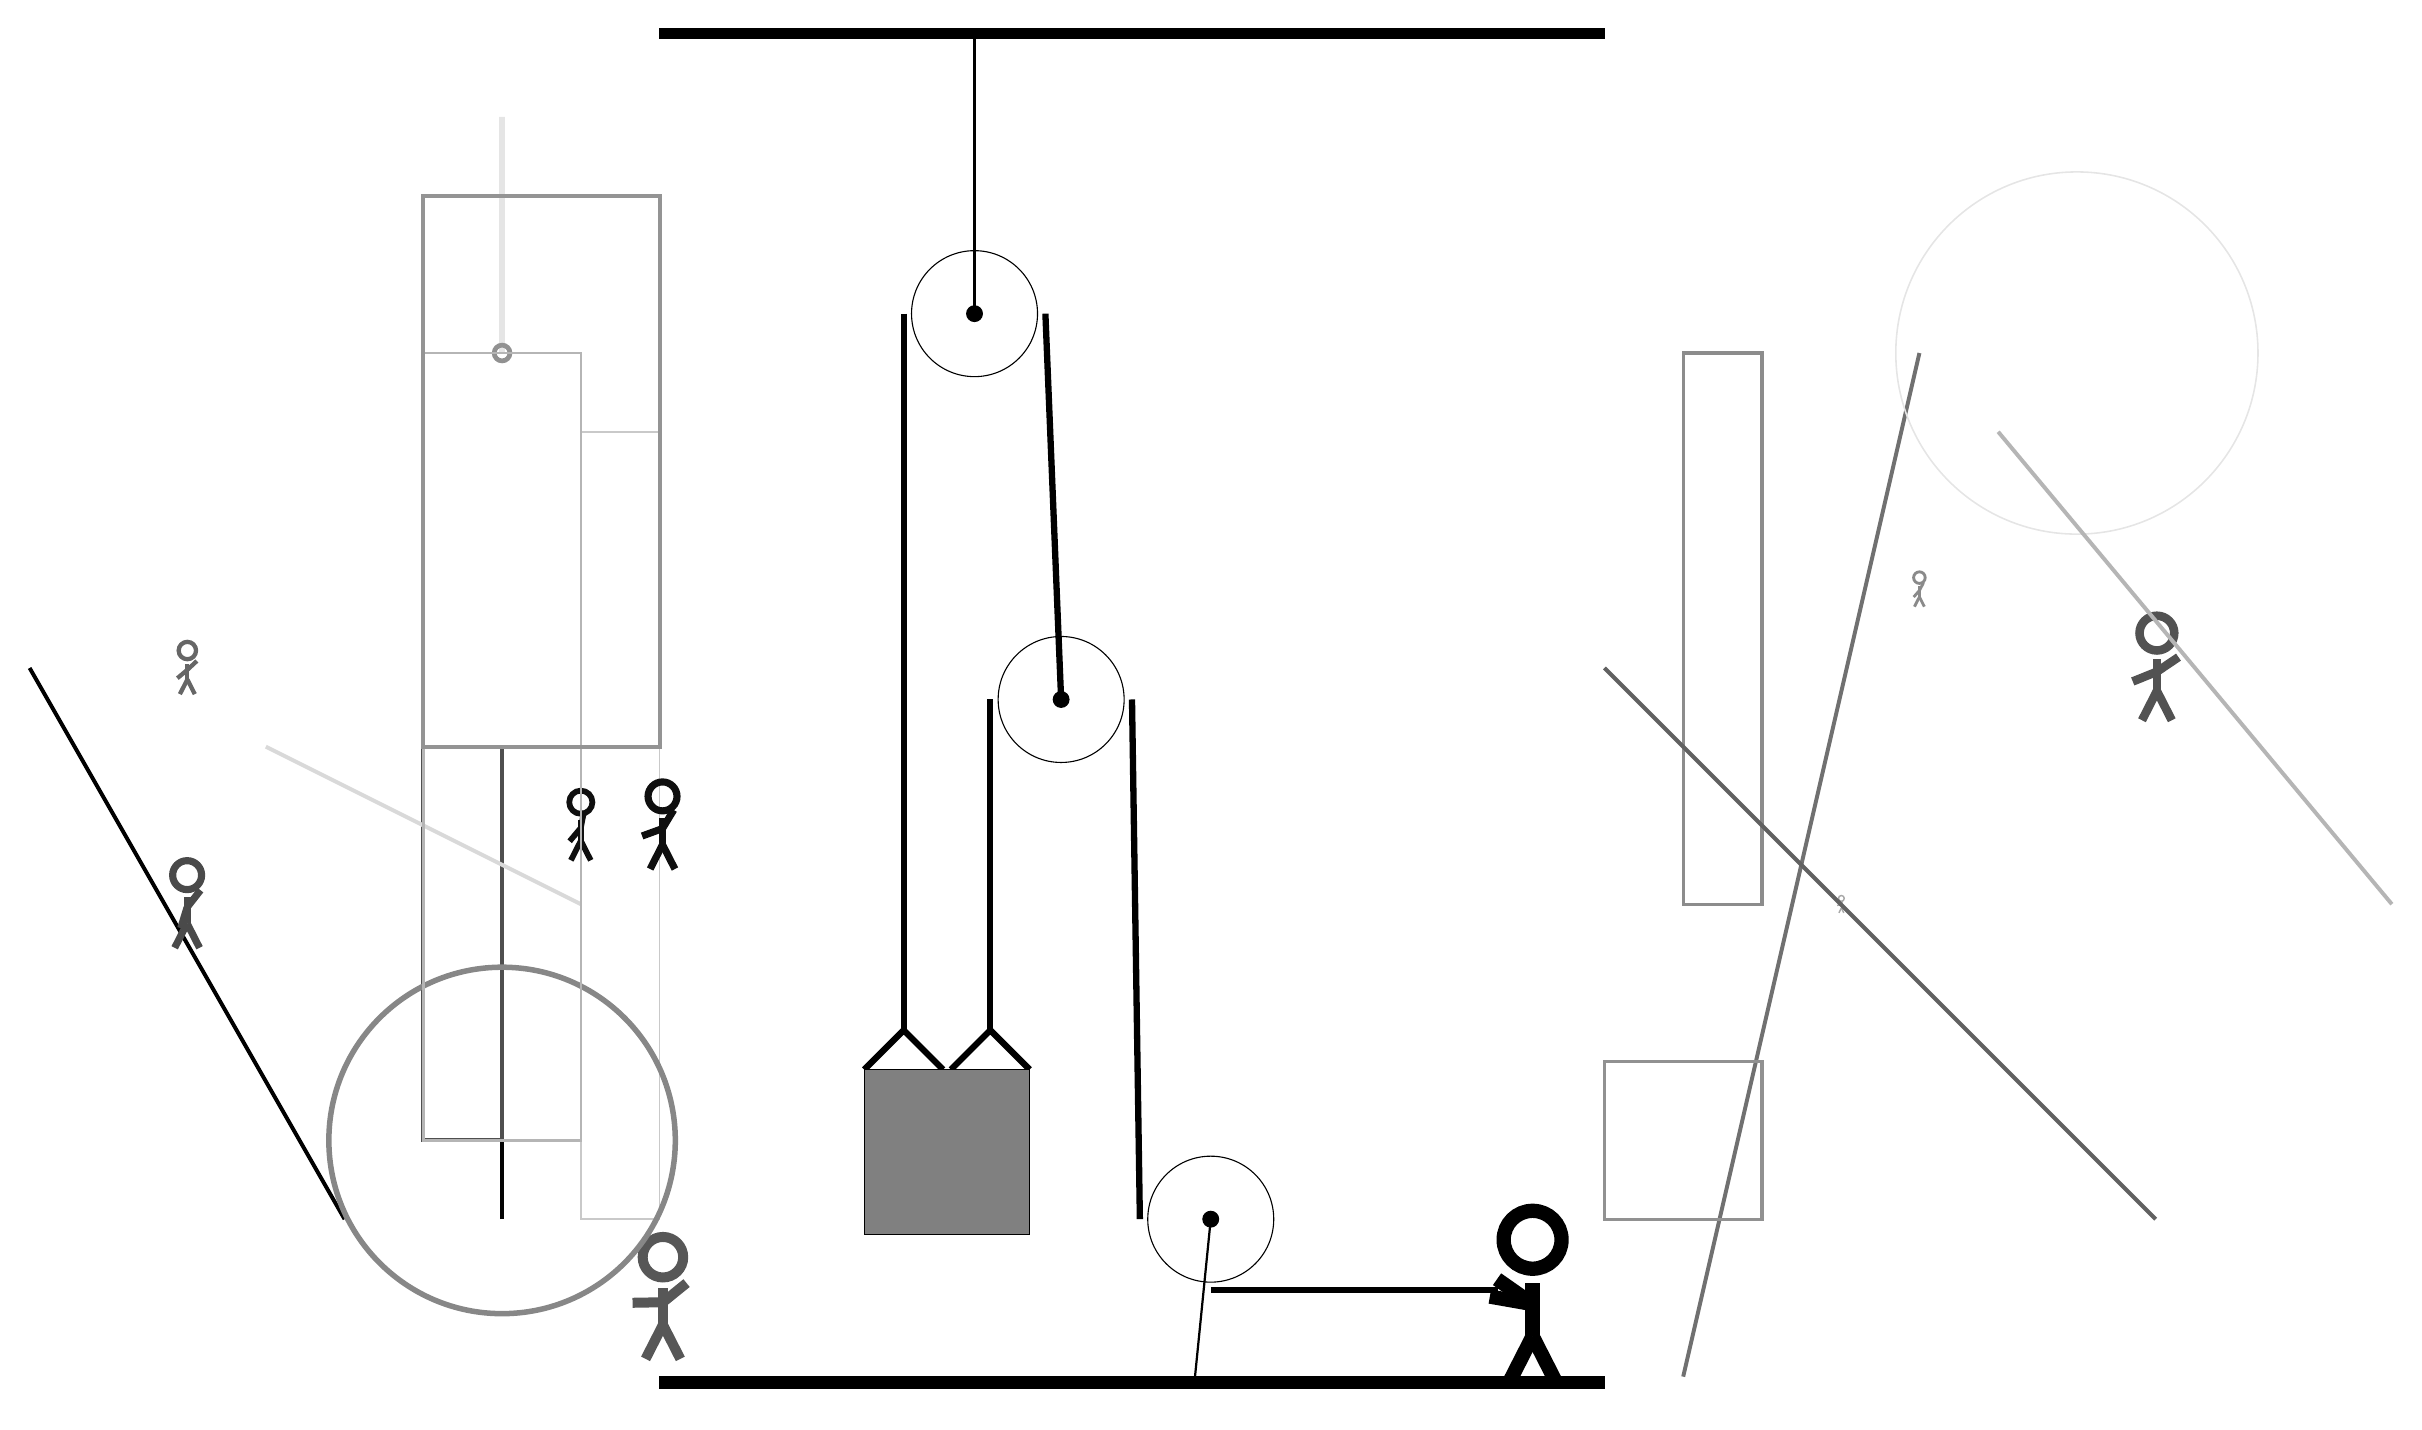
\begin{tikzpicture}
			%%%%% START %%%%%
			
			\draw[fill=black] (-2, 14) rectangle (10, 14.125);
			
			\draw (2, 10.5) circle (0.8);
			\draw[fill=black] (2, 10.5) circle (0.1);
			\draw[thick] (2, 10.5) -- (2, 14);
			
			\draw (3.1, 5.6) circle (0.8);
			\draw[fill=black] (3.1, 5.6) circle (0.1);
			
			\draw (5, -1) circle (0.8);
			\draw[fill=black] (5, -1) circle (0.1);
			\draw[thick] (5, -1) -- (4.8, -3);
			
			\draw[line width = 0.8mm]  (0.6, 0.9) -- (1.1, 1.4) -- (1.6, 0.9);
			\draw[line width = 0.8mm]  (1.7, 0.9) -- (2.2, 1.4) -- (2.7, 0.9);
			\draw[fill=black!50] (0.6, 0.9) rectangle (2.7, -1.2);
			
			\draw [line width=0.5mm, color=black!87](-4, -3) circle (0.0);
			
			\draw[line width=0.7mm, color=black!10] (-4, 10) rectangle (-4, 13);
			\node[line width=0.2mm, color=black!66] at (-2, -2) {\Strichmaxerl[7][1][39]};
			\draw[line width=0.5mm, color=black!99](-4, -1) -- (-4, 1);
			
			\draw[line width=0.5mm, color=black!56](11, -3) -- (14, 10);
			
			\draw [line width=0.2mm, color=black!10](16, 10) circle (2.3);
			
			\draw[line width=0.2mm, color=black!21] (-3, -1) rectangle (-2, 9);
			\node[line width=0.7mm, color=black!94] at (-2, 4) {\Strichmaxerl[5][20][59]};
			\draw[line width=0.4mm, color=black!43] (10, 1) rectangle (12, -1);
			\draw[line width=0.5mm, color=black!69] (-4, 5) rectangle (-5, 0);
			
			\draw[line width=0.5mm, color=black!100](-6, -1) -- (-10, 6);
			
			\node[line width=0.7mm, color=black!68] at (17, 6) {\Strichmaxerl[6][22][34]};
			\draw[line width=0.5mm, color=black!29](15, 9) -- (20, 3);
			\node[line width=0.2mm, color=black!94] at (-3, 4) {\Strichmaxerl[4][50][79]};
			\draw[line width=0.5mm, color=black!15](-7, 5) -- (-3, 3);
			\draw[line width=0.4mm, color=black!45] (11, 10) rectangle (12, 3);
			
			\draw [line width=0.7mm, color=black!47](-4, 0) circle (2.2);
			
			\node[line width=0.3mm, color=black!34] at (13, 3) {\Strichmaxerl[1][7][75]};
			\draw [line width=0.6mm, color=black!43](-4, 10) circle (0.1);
			
			\node[line width=0.7mm, color=black!60] at (-8, 6) {\Strichmaxerl[3][40][43]};
			\node[line width=0.3mm, color=black!71] at (-8, 3) {\Strichmaxerl[5][73][52]};
			\node[line width=0.6mm, color=black!46] at (14, 7) {\Strichmaxerl[2][49][62]};
			\draw[line width=0.3mm, color=black!29] (-3, 0) rectangle (-5, 10);
			\draw[line width=0.5mm, color=black!62](10, 6) -- (17, -1);
			\draw[line width=0.5mm, color=black!42] (-2, 12) rectangle (-5, 5);
			
			
			\draw[line width = 0.8mm] (1.1, 10.5) -- (1.1, 1.4);
			\centerarc[line width = 0.8mm](2, 10.5)(0:180:0.9);
			\draw[line width = 0.8mm] (2.9, 10.5) -- (3.1, 5.6);
			\draw[line width = 0.8mm] (2.2, 5.6) -- (2.2, 1.4);
			\centerarc[line width = 0.8mm](3.1, 5.6)(0:180:0.9);
			\draw[line width = 0.8mm] (4.0, 5.6) -- (4.1, -1);
			\centerarc[line width = 0.8mm](5, -1)(180:270:0.9);
			\draw[line width = 0.8mm] (5, -1.9) -- (8.65, -1.9);
			
			\node at (9, -2) {\Strichmaxerl[10][-35][170]};
			
			\draw[fill=black] (-2, -3) rectangle (10, -3.15);
			
			%%%%% END %%%%%
		\end{tikzpicture}
	\end{figure}	
\end{document}